%%%%%%%%%%%%%%%%%%%%%%%%%%%%%%%%%%%%%%%%%%%%%%%%%%%%%%%%%%%%%%%%%%%%%%%%%%%%%%%%%%
\begin{frame}[fragile]\frametitle{}
\begin{center}
{\Large Bitcoin}
\end{center}
\end{frame}

%%%%%%%%%%%%%%%%%%%%%%%%%%%%%%%%%%%%%%%%%%%%%%%%%%%%%%%%%%%%%%%%%%%%%%%%%%%%%%%%%%
\begin{frame}[fragile]\frametitle{Background}
In Crypto frameworks, there are 3 layers:
\begin{itemize}
\item Technology: Blockchain
\item Protocol/Coin: Bitcoin. 
\begin{itemize}
\item Protocol is a set of rules for participants to communicate, arrive at consensus and in general, govern the network, just like HTTP, TCP/IP, etc. 
\item Other protocols are: Ethereum, Neo, Ripple, etc. 
\item Each protocol has its on coin.
\end{itemize}
\item Token: functionality/idea based currency.
\begin{itemize}
\item ICO (Initial Coin Offering) is misleading as it is not about coin, but Token.
\item Tokens rely on Smart contracts. There are 100s of tokens on Ethereum (but only one coin, ie Eth)
\item Bitcoin has no token as it does not have Smart Contracts.
\end{itemize}
\end{itemize}
\end{frame}

%%%%%%%%%%%%%%%%%%%%%%%%%%%%%%%%%%%%%%%%%%%%%%%%%%%%%%%%%%%%%%%%%%%%%%%%%%%%%%%%%%
\begin{frame}[fragile]\frametitle{What is Bitcoin?}
\begin{itemize}
\item Bitcoin was invented by a pseudonymous person called Satoshi Nakamoto, in 2008, explained in a white (outline) paper (httos://bitcoin.org/bitcoin.pdf).
\item Code is Open sourced for anyone to copy, install and run the Bitcoin blockchain.
\item Bitcoin is a protocol on decentralized, peer-2-peer network to transact value/currency. No intermediary.
\item Bitcoin ecosystem: Nodes, Miners/users.
\end{itemize}
\end{frame}

%%%%%%%%%%%%%%%%%%%%%%%%%%%%%%%%%%%%%%%%%%%%%%%%%%%%%%%%%%%%%%%%%%%%%%%%%%%%%%%%%%
\begin{frame}[fragile]\frametitle{Bitcoin's Monetary Policy}
Entirely written in the code and has two main parts:
\begin{itemize}
\item Halving:Number of Bitcoins released after mining, is halved for each 4 years. It started with 50 BTC and now its 6.25. Thus total BTCs will grow infinitely but as the fractional is limited to 8 decimal points it will stop at 2040, with 21 Million BTCs. In addition there are separate transaction fees, which will go increasing.
\item Block Frequency: Average block times are: Bitcoin 10 minutes, Ethereum 15 sec, Ripple 3.5 sec etc.
\end{itemize}
\end{frame}

%%%%%%%%%%%%%%%%%%%%%%%%%%%%%%%%%%%%%%%%%%%%%%%%%%%%%%%%%%%%%%%%%%%%%%%%%%%%%%%%%%
\begin{frame}[fragile]\frametitle{Difficulty}
\begin{itemize}
\item Mining Target: the puzzle to solve. Meaning, how many leading 0's are being asked to get in the hash.
\item More the 0's more difficult it is.
\item 'XXXXX': 0 - 99999 ie 100k options. With '0XXXX': 0 - 9999 ie 10k options. Getting lesser options makes it a smaller pool to throw dart at.
\item For 18 leading 0's out of 64 characters. Total possible numbers: 16 x 16 x 16 \ldots 64 times = $16^{64}=1.15x10^{77}$. Total valid hashes with 18 leading 0s is $16^{64-18} = 2.45x10^{55}$ so prpbability is the ratio = $2x10^{-22}$ too small. (calculations not very correct?? as order is imp).
\item Difficulty = current target/ max target. It is adjusted every 2016 blocks (2 weeks). Mas target was the first target.
\end{itemize}
\end{frame}

%%%%%%%%%%%%%%%%%%%%%%%%%%%%%%%%%%%%%%%%%%%%%%%%%%%%%%%%%%%%%%%%%%%%%%%%%%%%%%%%%%
\begin{frame}[fragile]\frametitle{Mining Pool}
\begin{itemize}
\item Group of miners come together and form a syndicate.
\item They distribute the ranges to search into, say, 0 - 1B, 1B-2B, etc.
\item Once any one of them gets, it all share the rewards, based on hashing power submitted to the pool.
\item Generally a website or an organization, anyone can join.
\item They make individual getting into mining, very easy. 
\item China has/had 81\% hash power. Price of electricity decides profitability.
\end{itemize}

\begin{center}
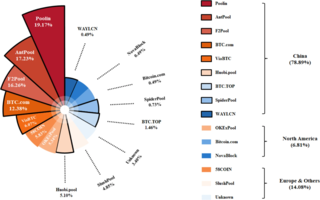
\includegraphics[width=0.6\linewidth,keepaspectratio]{blkchn_10}

{\tiny (Ref:``Bitcoin mining pools by location'' - Wikimedia - 20 May 2021)}
\end{center}
\end{frame}

%%%%%%%%%%%%%%%%%%%%%%%%%%%%%%%%%%%%%%%%%%%%%%%%%%%%%%%%%%%%%%%%%%%%%%%%%%%%%%%%%%
\begin{frame}[fragile]\frametitle{Nonce}
\begin{itemize}
\item Only 32 bit is allocated for Nonce number in a block, ie 0 to 4B ($2^{32}$).
\item Is this range good enough, so as to generate total block hash (64bit) with required number of leading 0's?
\item A modest miner can do 100 million hashes per second. So, 4 Billion will take 40 seconds.
\item There is another field called 	`timestamp' (unix time), so every second (even if you don't change Nonce) the block hash changes. So you have just 1 second to try whole Nonce range of 0-4B. So, you finish the Nonce range partially and start all over again in the next second.
\item But mining pools are fast, what happens when they finish computations within  a second?
\end{itemize}

\begin{center}
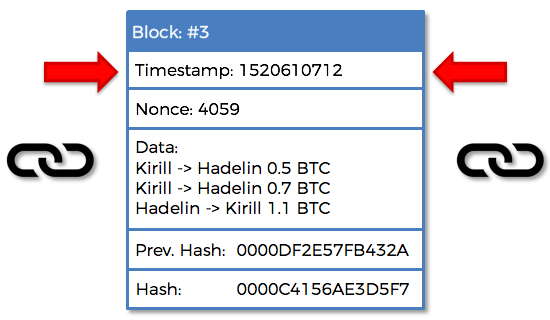
\includegraphics[width=0.4\linewidth,keepaspectratio]{blkchn_11}

{\tiny (Ref:``How does Bitcoin / Blockchain Mining work?'' by Kirill Eremenko  - Medium)}
\end{center}
\end{frame}


%%%%%%%%%%%%%%%%%%%%%%%%%%%%%%%%%%%%%%%%%%%%%%%%%%%%%%%%%%%%%%%%%%%%%%%%%%%%%%%%%%
\begin{frame}[fragile]\frametitle{How Miners pick Transactions?}
\begin{itemize}
\item Transactions keep on getting collected in a Mempool where Miners are registered. Like a staging area.
\item All these transactions are unconfirmed. Transaction fees are mentioned.
\item Miner picks high fees transactions.
\item Nonce computation starts, till required hash is achieved.
\item If you don't get the hash in required time,sa, 1 sec, then change the transactions. Repeat.
\item All this has been automated if you are part of a Mempool.
\end{itemize}

\begin{center}
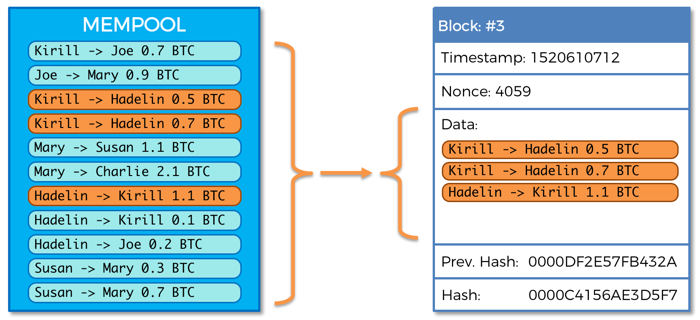
\includegraphics[width=0.6\linewidth,keepaspectratio]{blkchn_12}

{\tiny (Ref:``How does Bitcoin / Blockchain Mining work?'' by Kirill Eremenko  - Medium)}
\end{center}
\end{frame}

%%%%%%%%%%%%%%%%%%%%%%%%%%%%%%%%%%%%%%%%%%%%%%%%%%%%%%%%%%%%%%%%%%%%%%%%%%%%%%%%%%
\begin{frame}[fragile]\frametitle{Hardware}
\begin{itemize}
\item CPU: less than 10 million hashes per second
\item GPU : less than 1 Billion hashes per second
\item ASIC (Application Specific Integrated Circuit) very specific to calculate hashes: more than 1 trillion hashes per second
\item Cloud mining: pay per use.
\end{itemize}

\begin{center}
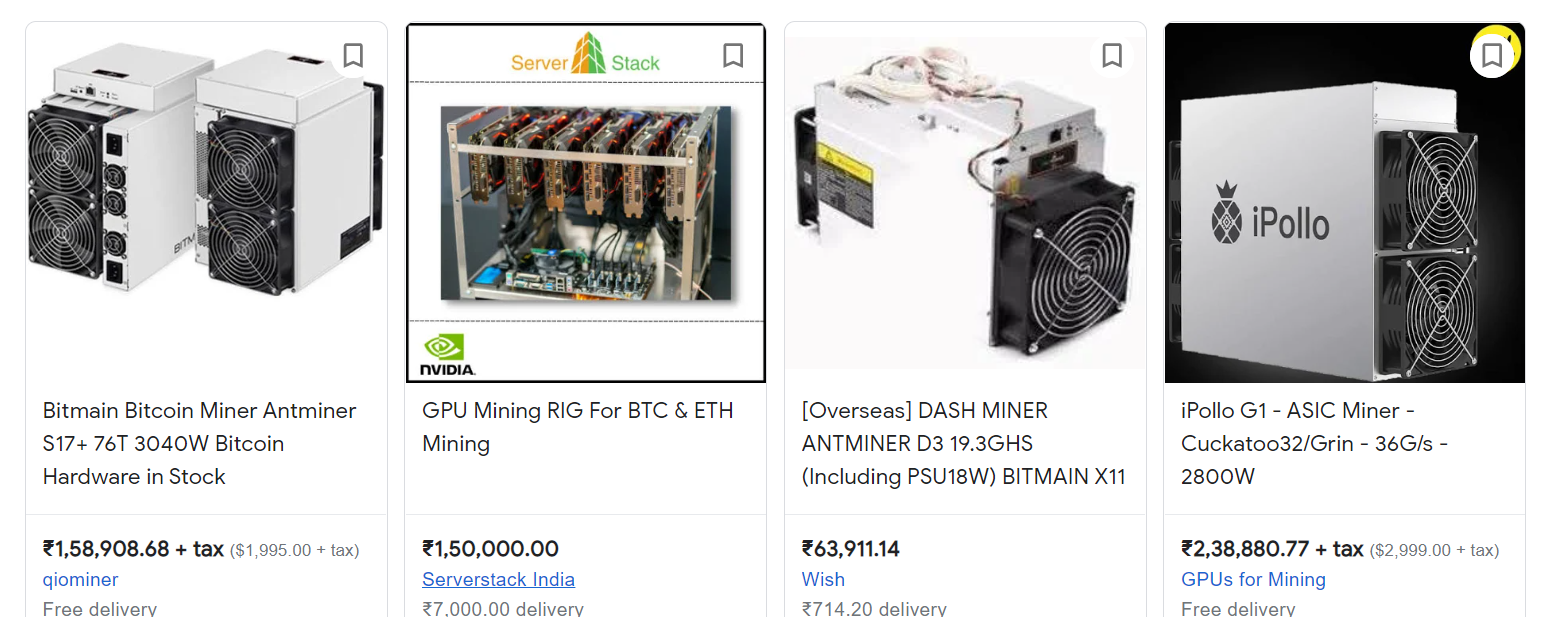
\includegraphics[width=0.8\linewidth,keepaspectratio]{blkchn_13}
\end{center}
\end{frame}

%%%%%%%%%%%%%%%%%%%%%%%%%%%%%%%%%%%%%%%%%%%%%%%%%%%%%%%%%%%%%%%%%%%%%%%%%%%%%%%%%%
\begin{frame}[fragile]\frametitle{51\% Attack}
\begin{itemize}
\item Hypothetical but feared that it will happen.
\item Cant attack any node of a blockchain, so its not about number of nodes, but about hash power.
\item Its about 51\% of mining is handled by malicious players. 
\item Such group gets hold of the blockchain and then does not rely back the changes to other nodes. Almost like cutting off.
\item As this group has more hash power, chains remain disconnected, and some time later start broadcasting again. As they are longer they win the further nodes and thus, own it. Nothing illegal as such, but the transaction they added may suffer double-spend. 
\item The lost transactions from trigonal chain go back to mempool just invalidating all those transactions.
\end{itemize}

\begin{center}
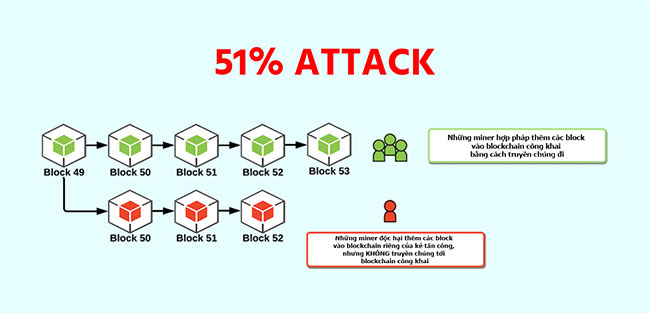
\includegraphics[width=0.4\linewidth,keepaspectratio]{blkchn_14}

{\tiny (Ref:``What is 51\% attack? How does 51\% attack work?'' - Tips Make)}
\end{center}

\end{frame}


%%%%%%%%%%%%%%%%%%%%%%%%%%%%%%%%%%%%%%%%%%%%%%%%%%%%%%%%%%%%%%%%%%%%%%%%%%%%%%%%%%
\begin{frame}[fragile]\frametitle{Transactions}
\begin{itemize}
\item UTXOs: Unspent Transactions Outputs. These transactions are like deferred expectations.
\item When a new transaction comes, you need to pair it with one/some of the earlier UTXOs.
\item There is no account to hold balance, all are just transactions, which will get evaluated every time.
\item Need to send all amount, if there is some balance left, make another transaction to put it in own account.
\end{itemize}

\begin{center}
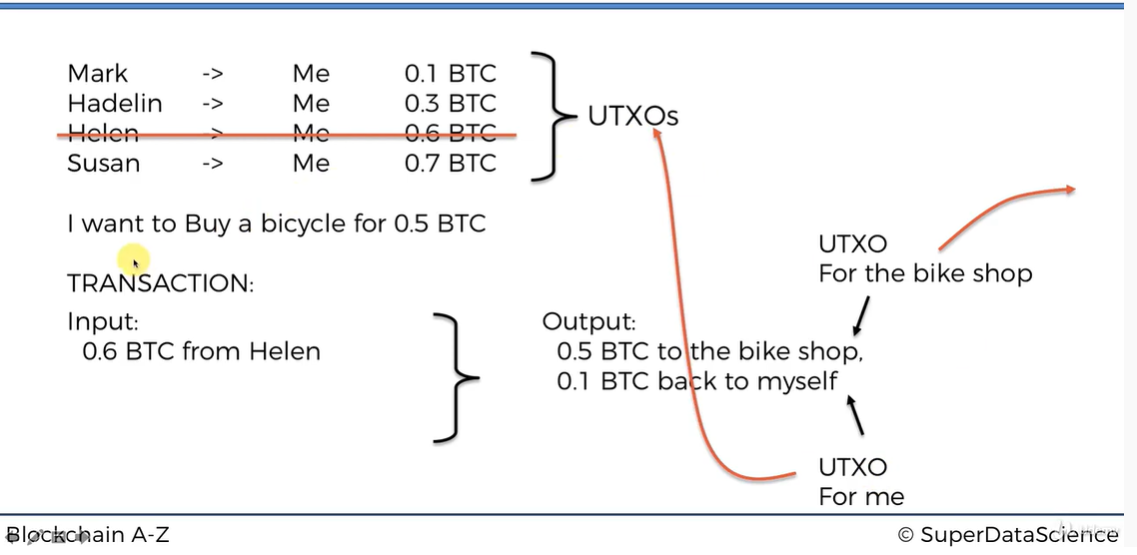
\includegraphics[width=0.6\linewidth,keepaspectratio]{blkchn_15}
\end{center}
\end{frame}

%%%%%%%%%%%%%%%%%%%%%%%%%%%%%%%%%%%%%%%%%%%%%%%%%%%%%%%%%%%%%%%%%%%%%%%%%%%%%%%%%%
\begin{frame}[fragile]\frametitle{Where Transactions Fees come from?}
\begin{itemize}
\item The unaccounted amount on the output side is considered as Transaction Fees and it goes to miner.
\item More the fees, more the chance of the transaction getting included.
\end{itemize}

\begin{center}
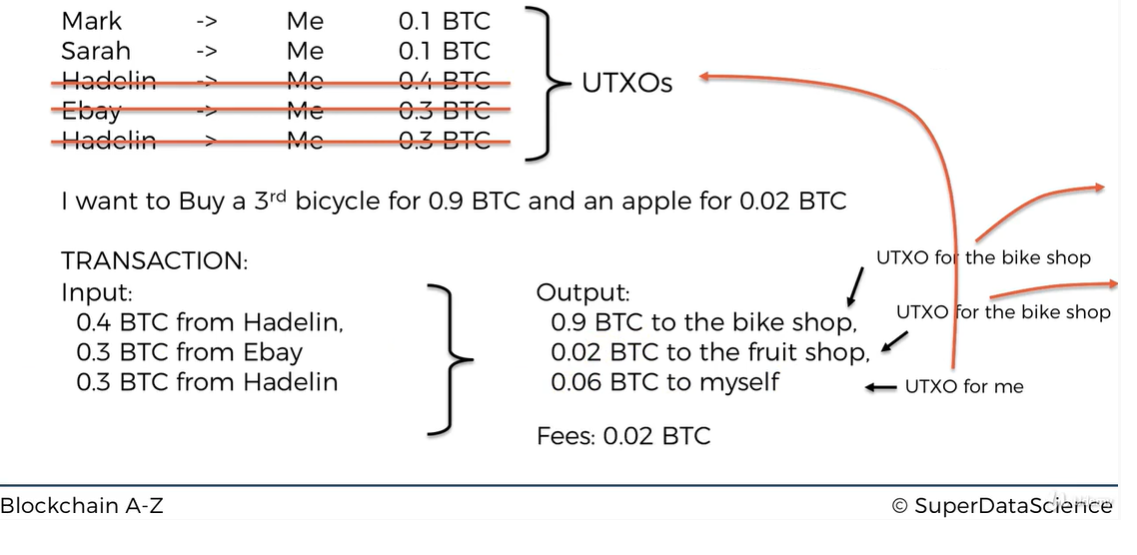
\includegraphics[width=0.6\linewidth,keepaspectratio]{blkchn_16}
\end{center}
\end{frame}

%%%%%%%%%%%%%%%%%%%%%%%%%%%%%%%%%%%%%%%%%%%%%%%%%%%%%%%%%%%%%%%%%%%%%%%%%%%%%%%%%%
\begin{frame}[fragile]\frametitle{How Wallets Work?}
\begin{itemize}
\item There isn't a balance value, then whats this wallet thing? On explorer page , you see the balance.
\item Wallets actually go through your transactions and then calculate your remaining UTXOs (ie Un-squared) on run time and show it to you.
\item Squared ones are shown with a block below.
\end{itemize}

\begin{center}
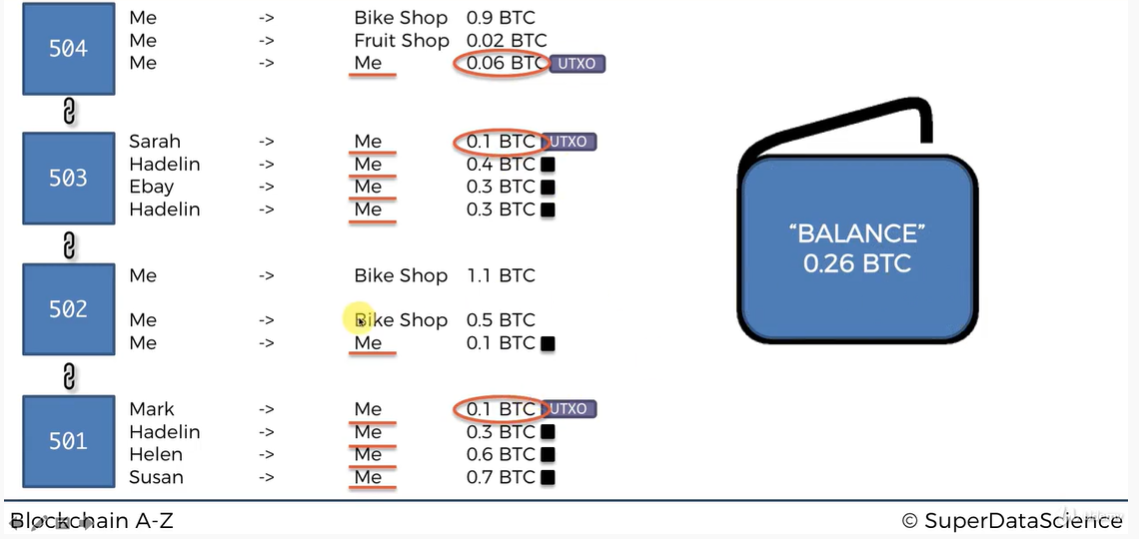
\includegraphics[width=0.6\linewidth,keepaspectratio]{blkchn_17}
\end{center}
\end{frame}

%%%%%%%%%%%%%%%%%%%%%%%%%%%%%%%%%%%%%%%%%%%%%%%%%%%%%%%%%%%%%%%%%%%%%%%%%%%%%%%%%%
\begin{frame}[fragile]\frametitle{Signatures}
\begin{itemize}
\item In transactions, Public Key is only visible, no other details, like name, city etc.
\item For adding transaction or deciphering transaction you need private key.
\item Any blockchain-account will give you PRIVATE key, with that you can generate PUBLIC key.
\item Anyone will need your PUBLIC key to send you money.
\item Transaction/message is signed using private key, which any verification agency can verify using public key.
\end{itemize}

\begin{center}
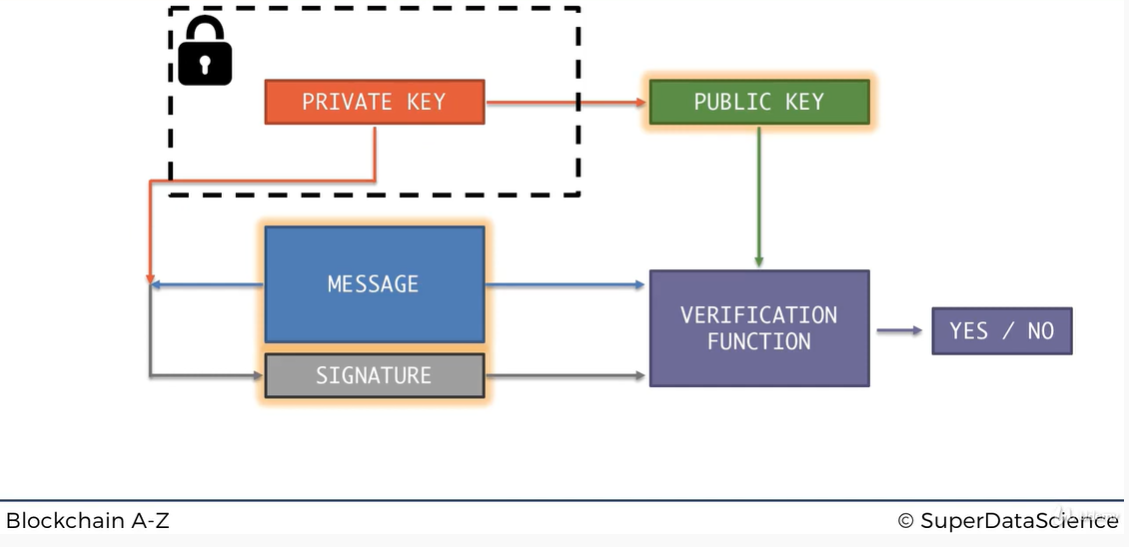
\includegraphics[width=0.6\linewidth,keepaspectratio]{blkchn_18}
\end{center}
\end{frame}

%%%%%%%%%%%%%%%%%%%%%%%%%%%%%%%%%%%%%%%%%%%%%%%%%%%%%%%%%%%%%%%%%%%%%%%%%%%%%%%%%%
\begin{frame}[fragile]\frametitle{Public Key vs Bitcoin Address}
\begin{itemize}
\item Bitcoin address is sha hash of Public Key.
\item Address is also public, and money can be sent to it as well, similar to Public Key.
\item So Bitcoin Address is just additional protection.
\end{itemize}

\begin{center}
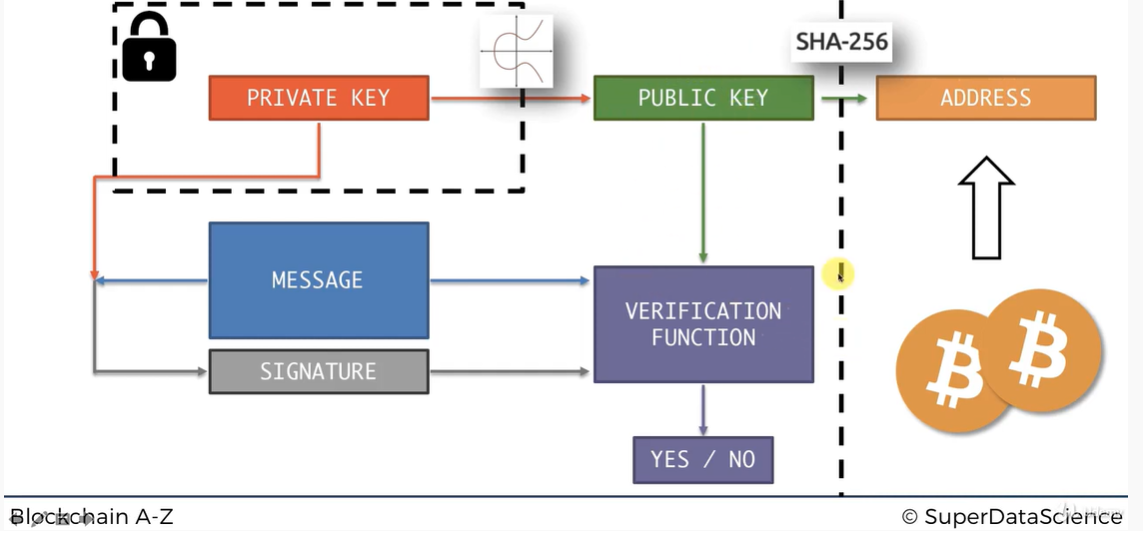
\includegraphics[width=0.6\linewidth,keepaspectratio]{blkchn_19}
\end{center}
\end{frame}

%%%%%%%%%%%%%%%%%%%%%%%%%%%%%%%%%%%%%%%%%%%%%%%%%%%%%%%%%%%%%%%%%%%%%%%%%%%%%%%%%%
\begin{frame}[fragile]\frametitle{}
\begin{center}
{\Large How Bitcoin Works?}
\end{center}
\end{frame}

%%%%%%%%%%%%%%%%%%%%%%%%%%%%%%%%%%%%%%%%%%%%%%%%%%%%%%%%%%%%%%%%%%%%%%%%%%%%%%%%%%
\begin{frame}[fragile]\frametitle{Background}
\begin{itemize}
\item Bitcoin blockchain is a giant track record of all the Bitcoin transactions that have ever occurred, all the way back to the very first Bitcoin transaction.
\end{itemize}


\end{frame}

%%%%%%%%%%%%%%%%%%%%%%%%%%%%%%%%%%%%%%%%%%%%%%%%%%%%%%%%%%%%%%%%%%%%%%%%%%%%%%%%%%
\begin{frame}[fragile]\frametitle{Step 1 — Transaction data}
\begin{itemize}
\item The blocks on the Bitcoin blockchain consist of approximately 1 MB of data each
\item The data is about Bitcoin transactions
\end{itemize}

\begin{center}
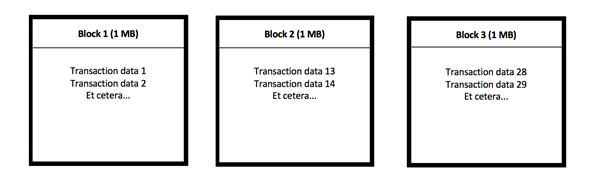
\includegraphics[width=0.8\linewidth,keepaspectratio]{blkchn_1}

{\tiny (Ref:``How does blockchain work in 7 steps — A clear and simple explanation.'' - Jimi S, Good Audience)}
\end{center}

\end{frame}

%%%%%%%%%%%%%%%%%%%%%%%%%%%%%%%%%%%%%%%%%%%%%%%%%%%%%%%%%%%%%%%%%%%%%%%%%%%%%%%%%%
\begin{frame}[fragile]\frametitle{Step 2 — Chaining the blocks (with a hash)}
\begin{itemize}
\item Let’s say block 1 registers two transactions, transaction 1 and transaction 2
\item Assume these fill up 1MB data limit.
\item This block of data now gets a signature for this specific string of data. Let’s say the signature is ‘X32’.
\item Similarly next set of transactions go to Block 2 with a signature '9BZ'.
\item Block 2 gets appended to the existing chain (ie Block 1) 
\item The signatures link the blocks to each other
\end{itemize}

\begin{center}
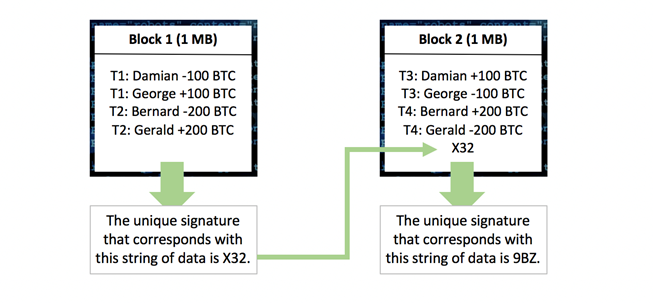
\includegraphics[width=0.6\linewidth,keepaspectratio]{blkchn_2}

{\tiny (Ref:``How does blockchain work in 7 steps — A clear and simple explanation.'' - Jimi S, Good Audience)}
\end{center}

\end{frame}

%%%%%%%%%%%%%%%%%%%%%%%%%%%%%%%%%%%%%%%%%%%%%%%%%%%%%%%%%%%%%%%%%%%%%%%%%%%%%%%%%%
\begin{frame}[fragile]\frametitle{Step 2 — Chaining the blocks (with a hash)}
\begin{itemize}
\item One more block comes (ie Block 3), it gets appended in a similar manner.
\item Now imagine if the data in block 1 is altered.
\item Damian now supposedly sent 500 Bitcoin to George instead of 100 Bitcoin.
\item Block 1's signature now changes, say it is now ‘W10’
\end{itemize}

\begin{center}
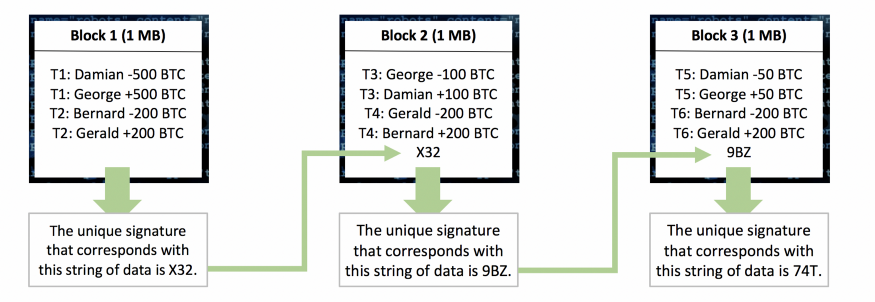
\includegraphics[width=0.6\linewidth,keepaspectratio]{blkchn_3}

{\tiny (Ref:``How does blockchain work in 7 steps — A clear and simple explanation.'' - Jimi S, Good Audience)}
\end{center}

\end{frame}

%%%%%%%%%%%%%%%%%%%%%%%%%%%%%%%%%%%%%%%%%%%%%%%%%%%%%%%%%%%%%%%%%%%%%%%%%%%%%%%%%%
\begin{frame}[fragile]\frametitle{Step 2 — Chaining the blocks (with a hash)}
\begin{itemize}
\item The signature W10 does not match the signature that was previously added to block 2 anymore. 
\item Block 1 and 2 are now considered no longer chained to each other. 
\item Blockchain rejects this change by shifting back to their previous record of the blockchain where all the blocks are still chained together (the record where Damian sent 100 BTC to George).
\item If you try to change pointer in Block 2, its data changes, this signature changes and so on
\item This means that altering a single block requires a new signature for every other block that comes after it all the way to the end of the chain. This is considered to be near impossible.
\end{itemize}

\begin{center}
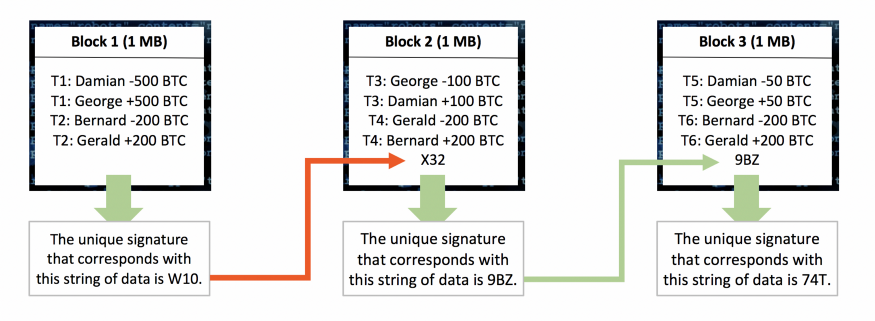
\includegraphics[width=0.6\linewidth,keepaspectratio]{blkchn_4}

{\tiny (Ref:``How does blockchain work in 7 steps — A clear and simple explanation.'' - Jimi S, Good Audience)}
\end{center}

\end{frame}

%%%%%%%%%%%%%%%%%%%%%%%%%%%%%%%%%%%%%%%%%%%%%%%%%%%%%%%%%%%%%%%%%%%%%%%%%%%%%%%%%%
\begin{frame}[fragile]\frametitle{Step 3 — How the signature (hash) is created}
\begin{itemize}
\item Signature is created by a cryptographic hash function. 
\item Takes any string of input and turns it into a unique 64-digit string of output.
\item e.g. ``761A7DD9CAFE34C7CDE6C1270E17F773025A61E511A56F700D415F0D3E199868''
\item If a single digit of the input changes, including a space, changing a capital letter or adding a period for example, the hash will be totally different.
\item But same string 'guarantees' same hash.
\end{itemize}

\begin{center}
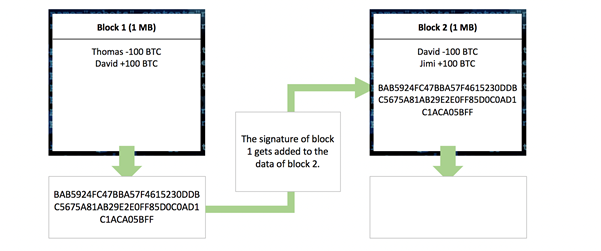
\includegraphics[width=0.6\linewidth,keepaspectratio]{blkchn_5}

{\tiny (Ref:``How does blockchain work in 7 steps — A clear and simple explanation.'' - Jimi S, Good Audience)}
\end{center}

\end{frame}

%%%%%%%%%%%%%%%%%%%%%%%%%%%%%%%%%%%%%%%%%%%%%%%%%%%%%%%%%%%%%%%%%%%%%%%%%%%%%%%%%%
\begin{frame}[fragile]\frametitle{Step 4 — When does the signature qualify, and who signs a block?}
\begin{itemize}
\item A block will only be accepted on the blockchain if its digital signature starts with — for example — a consecutive number of zeroes, Say, 10.
\item String of data of a block needs to be changed repeatedly until that specific string of data leads to a signature starting with ten zeroes. 
\item Because the transaction data and metadata (block number, timestamp, et cetera) need to stay the way they are, a small specific piece of data, called `nonce` is added to every block that has no purpose except for being changed repeatedly in order to find an eligible signature.
\item This is called mining and is what miners do. More compute you have (and luck), faster the process would be.
\end{itemize}

\begin{center}
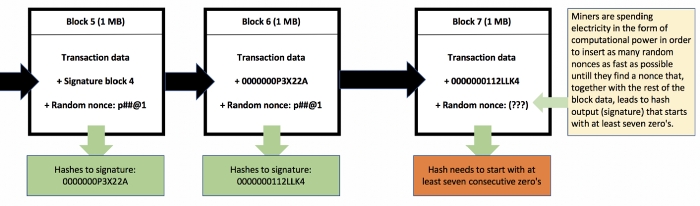
\includegraphics[width=0.6\linewidth,keepaspectratio]{blkchn_6}

{\tiny (Ref:``How does blockchain work in 7 steps — A clear and simple explanation.'' - Jimi S, Good Audience)}
\end{center}

\end{frame}

%%%%%%%%%%%%%%%%%%%%%%%%%%%%%%%%%%%%%%%%%%%%%%%%%%%%%%%%%%%%%%%%%%%%%%%%%%%%%%%%%%
\begin{frame}[fragile]\frametitle{Step 4 — When does the signature qualify, and who signs a block?}
\begin{itemize}
\item Any user on a blockchain network can participate in this process by downloading and starting the according mining software for that specific blockchain. 
\item When a user does this, they will simply put their computational power to work in order to try to solve the nonce for a block.
\item As you can see, the hash (signature) of this block and the hash of the previous block both start with a number of zeroes. 
\end{itemize}

\begin{center}
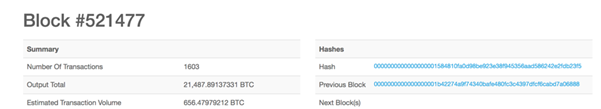
\includegraphics[width=0.6\linewidth,keepaspectratio]{blkchn_7}

{\tiny (Ref:``How does blockchain work in 7 steps — A clear and simple explanation.'' - Jimi S, Good Audience)}
\end{center}

\end{frame}

%%%%%%%%%%%%%%%%%%%%%%%%%%%%%%%%%%%%%%%%%%%%%%%%%%%%%%%%%%%%%%%%%%%%%%%%%%%%%%%%%%
\begin{frame}[fragile]\frametitle{Step 5 — How does this make the blockchain immutable?}
\begin{itemize}
\item Let’s say a corrupt miner has altered a block of transactions and is now trying to calculate new signatures for the subsequent blocks in order to have the rest of the network accept his change. 
\item The problem for him is, the rest of the network is also calculating new signatures for new blocks. 
\item The corrupt miner will have to calculate new signatures for these blocks too as they are being added to the end of the chain.
\item Unless the miner has more computational power than the rest of the network combined, he will never catch up with the rest of the network finding signatures.
\end{itemize}

\begin{center}
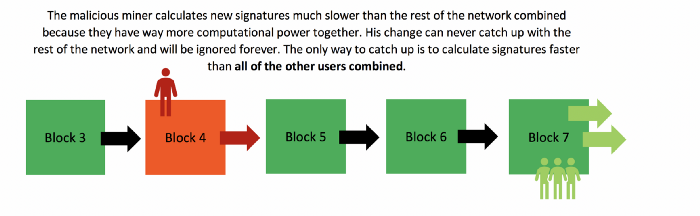
\includegraphics[width=0.6\linewidth,keepaspectratio]{blkchn_8}

{\tiny (Ref:``How does blockchain work in 7 steps — A clear and simple explanation.'' - Jimi S, Good Audience)}
\end{center}

\end{frame}

%%%%%%%%%%%%%%%%%%%%%%%%%%%%%%%%%%%%%%%%%%%%%%%%%%%%%%%%%%%%%%%%%%%%%%%%%%%%%%%%%%
\begin{frame}[fragile]\frametitle{Step 5 — How does this make the blockchain immutable?}
\begin{itemize}
\item What if a bad actor has more computational power than the rest of the network combined? Theoretically yes, this is possible. 
\item It is called a 51\% attack
\item It would not just require an immense amount of hardware, cooling equipment and storage space for the computational power, but also involves the risk of prosecution and, more importantly, would dramatically harm the ecosystem of the corresponding blockchain, rendering the potential returns in Bitcoin to drop significantly in value. 
\item This is also the reason that the more users participate in the mining process, the more secure a blockchain becomes.
\end{itemize}


\end{frame}

%%%%%%%%%%%%%%%%%%%%%%%%%%%%%%%%%%%%%%%%%%%%%%%%%%%%%%%%%%%%%%%%%%%%%%%%%%%%%%%%%%
\begin{frame}[fragile]\frametitle{Step 6 — How is the blockchain governed? Who determines the rules?}
\begin{itemize}
\item A governance model of democracy, so Majority wins.
\item It requires the majority of the computational power to create the longest version of the blockchain. 
\item This is also how an altered block is automatically rejected by the majority of the network.
\item On the Bitcoin blockchain, all transaction history and wallet balances are public (blockchain.info). 
\item Anyone can look up any wallet or transaction that has ever occurred all the way back to the first transaction that was ever made (on January 3rd, 2009). 
\item Although wallet balances can be checked by anyone publicly, the owners of those wallets remain largely unknown.
\end{itemize}


\end{frame}

%%%%%%%%%%%%%%%%%%%%%%%%%%%%%%%%%%%%%%%%%%%%%%%%%%%%%%%%%%%%%%%%%%%%%%%%%%%%%%%%%%
\begin{frame}[fragile]\frametitle{Final step, step 7 — Where does this leave cryptocurrencies?}
\begin{itemize}
\item Most cryptocurrencies are built upon their own blockchain protocol that may have different rules from the Bitcoin blockchain. 
\item Cryptocurrencies can however be given any kind of value, depending on their issuer. They could be referred to as ‘tokens’. 
\item Any sort of value can be attached to a ‘cryptocurrency’ token. 
\item All these cryptocurrency transactions are registered on various blockchains and can be exchanged online through cryptocurrency exchanges such as Binance. 
\end{itemize}


\end{frame}

